\documentclass[a4paper, 10pt]{article}
\usepackage{../CEDT-Homework-style}

\usepackage{amsmath}
\allowdisplaybreaks

\setlength{\headheight}{14.49998pt}


\newcommand{\zScoreTable}[1]{
    \par\noindent \textbf{z-table}
    \begin{table}[h]
        \centering
        \renewcommand{\arraystretch}{#1}
        \begin{tabular}{|c|cccccccccc|}
            \hline
            \textbf{z} & 0.0 & +0.1 & +0.2 & +0.3 & +0.4 & +0.5 & +0.6 & +0.7 & +0.8 & +0.9 \\
            \hline
            0.0 & 0.5000 & 0.5398 & 0.5793 & 0.6179 & 0.6554 & 0.6915 & 0.7258 & 0.7580 & 0.7881 & 0.8159 \\
            1.0 & 0.8413 & 0.8643 & 0.8849 & 0.9032 & 0.9192 & 0.9332 & 0.9452 & 0.9554 & 0.9641 & 0.9713 \\
            2.0 & 0.9773 & 0.9821 & 0.9861 & 0.9893 & 0.9918 & 0.9938 & 0.9953 & 0.9965 & 0.9974 & 0.9981 \\
            3.0 & 0.9987 & & & & & & & & & \\
            \hline
        \end{tabular}
        \caption{Standard Normal Distribution Table (z-table)}
        \label{tab:z-table}
    \end{table}
}


\begin{document}
\subject[2110205 - Statistics for Computer Engineering]
\hwtitle{5}{}{Week 6}{6733172621 Patthadon Phengpinij}{ChatGPT (for\,\LaTeX\,styling and grammar checking)}

% ================================================================================ %
\section{Week 6: Continuous Random Variables}
% ================================================================================ %



% ================================================================================ %
%                                    Problem 01                                    %
% ================================================================================ %
\begin{problem}
For each statement below, determine if it is True or False.
\begin{subproblems}
    \item The value of a Probability Density Function (PDF), \( f(x) \), can be greater than 1.
    \item The value of a Cumulative Distribution Function (CDF), \( F(x) \), can be greater than 1.
    \item The integral of a valid PDF, \( \int_{-\infty}^{\infty} f(x)\,dx \), over its entire range must equal 1.
    \item For any continuous random variable \( X \), the probability \( P(X = c) \) is always 0.
\end{subproblems}
\end{problem}

\begin{solution}
\begin{subproblems}
    \item \boxed{\textbf{True.}} A PDF can take values greater than 1, as long as the total area under the curve equals 1.
    \item \boxed{\textbf{False.}} A CDF must always be between 0 and 1, inclusive.
    \item \boxed{\textbf{True.}} The integral of a valid PDF over its entire range must equal 1, representing the total probability.
    \item \boxed{\textbf{True.}} For continuous random variables, the probability of taking any specific value is 0, since there are infinitely many possible values.
\end{subproblems}
\end{solution}
% ================================================================================ %


% ================================================================================ %
%                                    Problem 02                                    %
% ================================================================================ %
\begin{problem}
A continuous random variable \( X \) has the following piecewise PDF:
\[
f(x) = \begin{cases}
cx & 0 \leq x \le 2 \\
c\paren{4 - x} & 2 \leq x \leq 4 \\
0 & \text{otherwise}
\end{cases}
\]
\begin{subproblems}
    \item Find the value of c that makes \( f(x) \) a valid PDF.
    \item Sketch the graph of the PDF.
\end{subproblems}
\end{problem}

\begin{solution}
For a valid PDF, the total area under the curve must equal 1. We can find \( c \) by integrating \( f(x) \) over its entire range and setting the integral equal to 1.
\begin{align*}
    1 = \int_{-\infty}^{\infty} f(x)\,dx &= \int_{0}^{2} cx\,dx + \int_{2}^{4} c(4 - x)\,dx \\
    &= c \sqbracket{\frac{x^2}{2}}_{0}^{2} + c \sqbracket{4x - \frac{x^2}{2}}_{2}^{4} \\
    &= c \sqbracket{\frac{2^2}{2} - 0 + \paren{4(4) - \frac{4^2}{2}} - \paren{4(2) - \frac{2^2}{2}}} \\
    &= c \sqbracket{2 + (16 - 8) - (8 - 2)} \\
    1 &= c \sqbracket{2 + 8 - 6} = 4c \\
\end{align*}
Thus, the value of \( c \) that would make this PDF valid is: \( \boxed{c = \frac{1}{4}} \; \textbf{a).} \)

This PDF would be:
\[
f(x) = \begin{cases}
    \tfrac{1}{4}x & 0 \leq x \le 2 \\
    \tfrac{1}{4}(4 - x) & 2 \leq x \leq 4 \\
    0 & otherwise
\end{cases}
\]

\textbf{b).} The graph of the PDF is as follows:
\begin{center}
    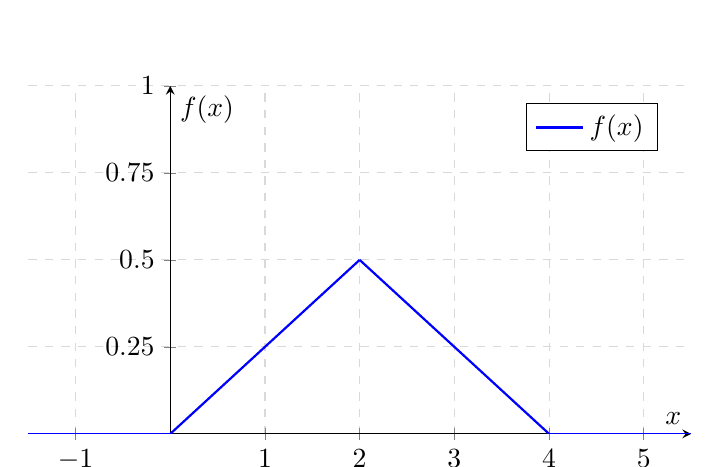
\begin{tikzpicture}
        \begin{axis}[
            axis lines = middle,
            xlabel = \(x\),
            ylabel = {\(f(x)\)},
            ymin = 0, ymax = 1,
            xmin = -1.5, xmax = 5.5,
            xtick = {-1, 0, 1, 2, 3, 4, 5},
            ytick = {0, 0.25, 0.5, 0.75, 1},
            grid = major,
            grid style = {dashed, gray!30},
            width = 10cm, height = 6cm,
            domain = 0:4,
            samples = 100,
            legend style = {at={(0.95,0.95)}, anchor=north east},
            legend cell align = left
        ]
            \addplot[blue, thick, domain=-1.5:0] {0};
            \addplot[blue, thick, domain=0:2] {0.25*x};
            \addplot[blue, thick, domain=2:4] {0.25*(4 - x)};
            \addplot[blue, thick, domain=4:5.5] {0};
            \addlegendentry{\( f(x) \)}
        \end{axis}
    \end{tikzpicture}
\end{center}
\end{solution}
% ================================================================================ %


% ================================================================================ %
%                                    Problem 03                                    %
% ================================================================================ %
\begin{problem}
Using the PDF from Problem 2:
\begin{subproblems}
    \item Calculate the probability \( P(X > 2.5) \).
    \item Derive the Cumulative Distribution Function (CDF), \( F(x) \).
\end{subproblems}
\end{problem}

\begin{solution}
From the previous problem, we have the PDF:
\[
f(x) = \begin{cases}
    \tfrac{1}{4}x & 0 \leq x \le 2 \\
    \tfrac{1}{4}(4 - x) & 2 \leq x \leq 4 \\
    0 & otherwise
\end{cases}
\]

To calculate \( P(X > 2.5) \), we integrate the PDF from 2.5 to 4:
\begin{align*}
    P(X > 2.5) &= \int_{2.5}^{\infty} f(x)\,dx \\
    &= \int_{2.5}^{4} f(x)\,dx + \int_{4}^{\infty} f(x)\,dx \\
    &= \int_{2.5}^{4} \frac{1}{4}(4 - x)\,dx + \int_{4}^{\infty} 0\,dx \\
    &= \frac{1}{4} \sqbracket{4x - \frac{x^2}{2}}_{2.5}^{4} + 0 \\
    &= \frac{1}{4} \sqbracket{(16 - 8) - (10 - 3.125)} \\
    &= \frac{1}{4} \sqbracket{8 - 6.875} \\
    P(X > 2.5) &= \frac{1}{4} \cdot 1.125 = 0.28125
\end{align*}
Thus, \( P(X > 2.5) = \boxed{0.28125} \; \textbf{a).} \)

\vspace{4mm}

To derive the CDF, \( F(x) \), we integrate the PDF from the lower limit to \( x \). \\
Considering the piecewise nature of the PDF, we have:
\begin{align*}
    f(x) &= \begin{cases}
        0 & x \le 0 \\
        \frac{1}{4}x & 0 \leq x \le 2 \\
        \frac{1}{4}(4 - x) & 2 \leq x \le 4 \\
        0 & x \geq 4
    \end{cases} \\ \
    F(x) &= \begin{cases}
        0 & x \le 0 \\
        \int_{0}^{x} \frac{1}{4}t\,dt & 0 \leq x \le 2 \\
        \int_{0}^{2} \frac{1}{4}t\,dt + \int_{2}^{x} \frac{1}{4}(4 - t)\,dt & 2 \leq x \le 4 \\
        1 & x \geq 4
    \end{cases} \\
\end{align*}
Calculating the integrals:
\begin{align*}
    \int_{0}^{x} \frac{1}{4}t\,dt &= \frac{1}{4} \cdot \sqbracket{\frac{t^2}{2}}_{0}^{x} \\
    &= \frac{1}{4} \cdot \frac{x^2}{2} \\
    \int_{0}^{x} \frac{1}{4}t\,dt &= \frac{x^2}{8} \\
\end{align*}
And:
\begin{align*}
    \int_{2}^{x} \frac{1}{4}(4 - t)\,dt &= \frac{1}{4} \cdot \sqbracket{4t - \frac{t^2}{2}}_{2}^{x} \\
    &= \frac{1}{4} \cdot \paren{(4x - \frac{x^2}{2}) - (8 - 2)} \\
    &= \frac{1}{4} \cdot (4x - \frac{x^2}{2} - 6) \\
    \int_{2}^{x} \frac{1}{4}(4 - t)\,dt &= x - \frac{x^2}{8} - \frac{3}{2} \\
\end{align*}

Thus, the CDF \( F(x) \) is:
\[
F(x) = \begin{cases}
    0 & x < 0 \\
    \frac{x^2}{8} & 0 \leq x \le 2 \\
    \paren{\frac{x^2}{8}}_{x=2} + \paren{x - \frac{x^2}{8} - \frac{3}{2}} & 2 \leq x \le 4 \\
    1 & x \geq 4
\end{cases}
\]
\[
\boxed{F(x) = \begin{cases}
    0 & x < 0 \\
    \frac{x^2}{8} & 0 \leq x < 2 \\
    x - \frac{x^2}{8} - 1 & 2 \leq x < 4 \\
    1 & x \geq 4
\end{cases}} \; \textbf{b).}
\]
\end{solution}
% ================================================================================ %

\newpage

% ================================================================================ %
%                                    Problem 04                                    %
% ================================================================================ %
\begin{problem}
Using the CDF from Problem 3, find the median of the random variable \( X \).
\end{problem}

\begin{solution}
From the previous problem, we have the CDF:
\[
F(x) = \begin{cases}
    0 & x \leq 0 \\
    \frac{x^2}{8} & 0 \leq x \leq 2 \\
    x - \frac{x^2}{8} - 1 & 2 \leq x < 4 \\
    1 & x \geq 4
\end{cases}
\]

For a random variable \( X \), the median is the value \( m \) such that \( F(m) = 0.5 \).
To find the median, we need to solve for \( m \) in the equation \( F(m) = 0.5 \).
We consider the piecewise nature of the CDF:
\begin{enumerate}
    \item For \( 0 \leq m \leq 2 \):
    \[
    F(m) = \frac{m^2}{8} = 0.5
    \]
    Solving for \( m \):
    \[
    m^2 = 4 \implies m = 2 \implies m \in [0, 2], \underline{\textbf{valid.}}
    \]
    
    \item For \( 2 \leq m \leq 4 \):
    \[
    F(m) = m - \frac{m^2}{8} - 1 = 0.5
    \]
    Solving for \( m \):
    \[
    m - \frac{m^2}{8} = 1.5
    \]
    Multiplying through by 8 to eliminate the fraction:
    \[
    8m - m^2 = 12
    \]
    Rearranging gives us a quadratic equation:
    \[
    m^2 - 8m + 12 = 0
    \]
    Factoring:
    \[
    (m - 6)(m - 2) = 0
    \]
    Thus, \( m = 6 \) or \( m = 2 \). Since we are considering the interval \( [2, 4] \), we have:
    \[
    m = 2 \implies m \in [2, 4], \underline{\textbf{valid.}}
    \]
\end{enumerate}

Thus, the median of the random variable \( X \) is \( \boxed{2} \).
\end{solution}
% ================================================================================ %

\newpage

% ================================================================================ %
%                                    Problem 05                                    %
% ================================================================================ %
\begin{problem}
A shuttle bus arrives at a student dormitory at a random time within a 15-minute window, from 8:00 AM to 8:15 AM.
Let \( T \) be the student's waiting time in minutes if they arrive at exactly 8:00 AM.
\begin{subproblems}
    \item What is the distribution of \( T \)? (Specify type and parameters).
    \item What is the probability that a student waits for more than 10 minutes?
\end{subproblems}
\end{problem}

\begin{solution}
\textbf{a).} The waiting time \( T \) follows a uniform distribution over the interval [0, 15] minutes.
Thus, we can denote this as: \( T \sim \text{Uniform}(0, 15) \)

\vspace{3mm}

\textbf{b).} To find the probability that a student waits for more than 10 minutes: \( P(T > 10) \).
The PDF of a uniform distribution over the interval [a, b] is given by:
\[
f_T(t) = \begin{cases}
    \frac{1}{b-a} & a \leq t \leq b \\
    0 & \text{otherwise}
\end{cases}
\]
For our case, \( a = 0 \) and \( b = 15 \), so the PDF is:
\[
f_T(t) = \begin{cases}
    \frac{1}{15} & 0 \leq t \leq 15 \\
    0 & \text{otherwise}
\end{cases}
\]
To find \( P(T > 10) \), we can integrate the PDF from 10 to 15:
\[
P(T > 10) = \int_{10}^{15} f_T(t) \, dt = \int_{10}^{15} \frac{1}{15} \, dt = \frac{1}{15} \cdot (15 - 10) = \frac{5}{15} = \frac{1}{3}
\]
Thus, the probability that a student waits for more than 10 minutes is \( \boxed{\frac{1}{3}} \).
\end{solution}
% ================================================================================ %


% ================================================================================ %
%                                    Problem 06                                    %
% ================================================================================ %
\begin{problem}
For the shuttle bus scenario in Problem 5:
\begin{subproblems}
    \item What is the expected waiting time, \( \text{E}[T] \)?
    \item What is the variance of the waiting time, \( \text{Var}(T) \)?
\end{subproblems}
\end{problem}

\begin{solution}
From Problem 5, we know that \( T \sim \text{Uniform}(0, 15) \).

\vspace{3mm}

For a uniform distribution \( \text{Uniform}(a, b) \):
\begin{itemize}
    \item The expected value \( \text{E}[X] = \frac{a + b}{2} \)
    \item The variance \( \text{Var}(X) = \frac{(b - a)^2}{12} \)
\end{itemize}

The expected waiting time \( \text{E}[T] \) is:
\[ \text{E}[T] = \frac{0 + 15}{2} = \frac{15}{2} = \boxed{7.5 \text{ minutes}} \; \textbf{a).} \]
The variance of the waiting time \( \text{Var}(T) \) is:
\[ \text{Var}(T) = \frac{(15 - 0)^2}{12} = \frac{225}{12} = \boxed{18.75 \text{ minutes}^2}  \; \textbf{b).} \]
\end{solution}
% ================================================================================ %


% ================================================================================ %
%                                    Problem 07                                    %
% ================================================================================ %
\begin{tosubmit}
\problem
For the shuttle bus scenario in Problem 5, what is the \( 80^\text{th} \) percentile of the waiting time?
In other words, find the time \( t \) (in minutes) such that 80\% of waiting times are less than \( t \).

\vspace{3mm}

\par\noindent\submitsolution
From Problem 5, we know that \( T \sim \text{Uniform}(0, 15) \). \newline
The CDF of a uniform distribution \( \text{Uniform}(a, b) \) is given by:
\[
F_T(t) = \begin{cases}
    0 & t < a \\
    \frac{t - a}{b - a} & a \leq t \leq b \\
    1 & t > b
\end{cases}
\]
For our case, \( a = 0 \) and \( b = 15 \), so the CDF is:
\[
F_T(t) = \begin{cases}
    0 & t < 0 \\
    \frac{t}{15} & 0 \leq t \leq 15 \\
    1 & t > 15
\end{cases}
\]
To find the 80th percentile, we need to solve for \( t \) in the equation \( F_T(t) = 0.8 \):
\[\frac{t}{15} = 0.8 \]
Solving for \( t \):
\[ t = 0.8 \times 15 = 12 \]
Thus, the 80th percentile of the waiting time is \( \boxed{12 \text{ minutes}} \).
\end{tosubmit}
% ================================================================================ %


% ================================================================================ %
%                                    Problem 08                                    %
% ================================================================================ %
\begin{problem}
The lifespan of a particular brand of hard drive, in years, follows an exponential
distribution with a mean of 4 years.
\begin{subproblems}
    \item What is the value of the parameter \( \lambda \) for this distribution?
    \item What is the probability that a new hard drive lasts for less than 1 year?
\end{subproblems}
\end{problem}

\begin{solution}
For an exponential distribution, the mean \( \mu \) is given by:
\[ \mu = \frac{1}{\lambda} \]
Given that the mean lifespan of the hard drive is 4 years, we can find \( \lambda \):
\[ 4 = \frac{1}{\lambda} \implies \lambda = \boxed{\frac{1}{4}} \; \textbf{a).} \]

The PDF of an exponential distribution is given by:
\[ f(x) = \lambda e^{-\lambda x} \text{ for } x \geq 0 \]
To find the probability that a new hard drive lasts for less than 1 year, we calculate:
\[ P(X < 1) = \int_{0}^{1} f(x)\,dx = \int_{0}^{1} \frac{1}{4} e^{-\frac{1}{4} x}\,dx = \sqbracket{-e^{-\frac{1}{4} x}}_{0}^{1} = -e^{-\frac{1}{4}} + e^{0} = 1 - e^{-\frac{1}{4}} \approx 0.2212 \]
Thus, the probability that a new hard drive lasts for less than 1 year is \( \boxed{1 - e^{-\frac{1}{4}}} \; \textbf{b).} \)
\end{solution}
% ================================================================================ %


% ================================================================================ %
%                                    Problem 09                                    %
% ================================================================================ %
\begin{tosubmit}
\problem
For the hard drive in Problem 8, you discover an old one that is still working after 3 years.
What is the probability that it will continue to work for at least another 4 years?

\par\noindent\submitsolution
From Problem 8, we know that the lifespan of the hard drive follows an exponential distribution with parameter \( \lambda = \frac{1}{4} \).

\vspace{2mm}

The exponential distribution has the memoryless property, which means that the probability of surviving an additional time period is independent of how long it has already survived.

\vspace{2mm}

Thus, we need to find \( P(X > 7 \mid X > 3) \), which is equivalent to \( P(X > 4) \) due to the memoryless property.
\[ P(X > 4) = e^{-\lambda \cdot 4} = e^{-\frac{1}{4} \cdot 4} = e^{-1} \approx 0.3679 \]
Thus, the probability that the hard drive will continue to work for at least another 4 years is \( \boxed{e^{-1}} \).
\end{tosubmit}
% ================================================================================ %


% ================================================================================ %
%                                    Problem 10                                    %
% ================================================================================ %
\begin{problem}
What is the \textbf{median} lifespan of the hard drives from Problem 8?
Is this value smaller or larger than the mean lifespan, and why does this make intuitive sense for this distribution?
\end{problem}

\begin{solution}
From Problem 8, we know that the lifespan of the hard drive follows an exponential distribution with parameter \( \lambda = \frac{1}{4} \).

\vspace{2mm}

The CDF of an exponential distribution is given by:
\[ F(x) = 1 - e^{-\lambda x} \text{ for } x \geq 0 \]

To find the median lifespan, we need to solve for \( m \) in the equation \( F(m) = 0.5 \):
\begin{align*}
    0.5 &= 1 - e^{-\frac{1}{4} m} \\
    e^{-\frac{1}{4} m} &= 0.5 \\
    -\frac{1}{4} m &= \ln(0.5) \\
    m &= -4 \ln(0.5) \\
    m &= 4 \ln(2)
\end{align*}
Thus, the median lifespan of the hard drives is \( \boxed{4 \ln(2) \approx 2.7726 \text{ years}} \).
\end{solution}
% ================================================================================ %

\newpage

% ================================================================================ %
%                                    Problem 11                                    %
% ================================================================================ %
\begin{tosubmit}
\problem
The final exam scores for a large statistics class are normally distributed with a
mean of 72 and a standard deviation of 12.
\begin{subproblems}
    \item What is the probability that a randomly selected student scores between 65 and 85?
    \item What is the probability a student scores exactly 80.00?
\end{subproblems}

\par\noindent\submitsolution
From the z-table provided, we can use the standard normal distribution to find the required probabilities.
\begin{center}
    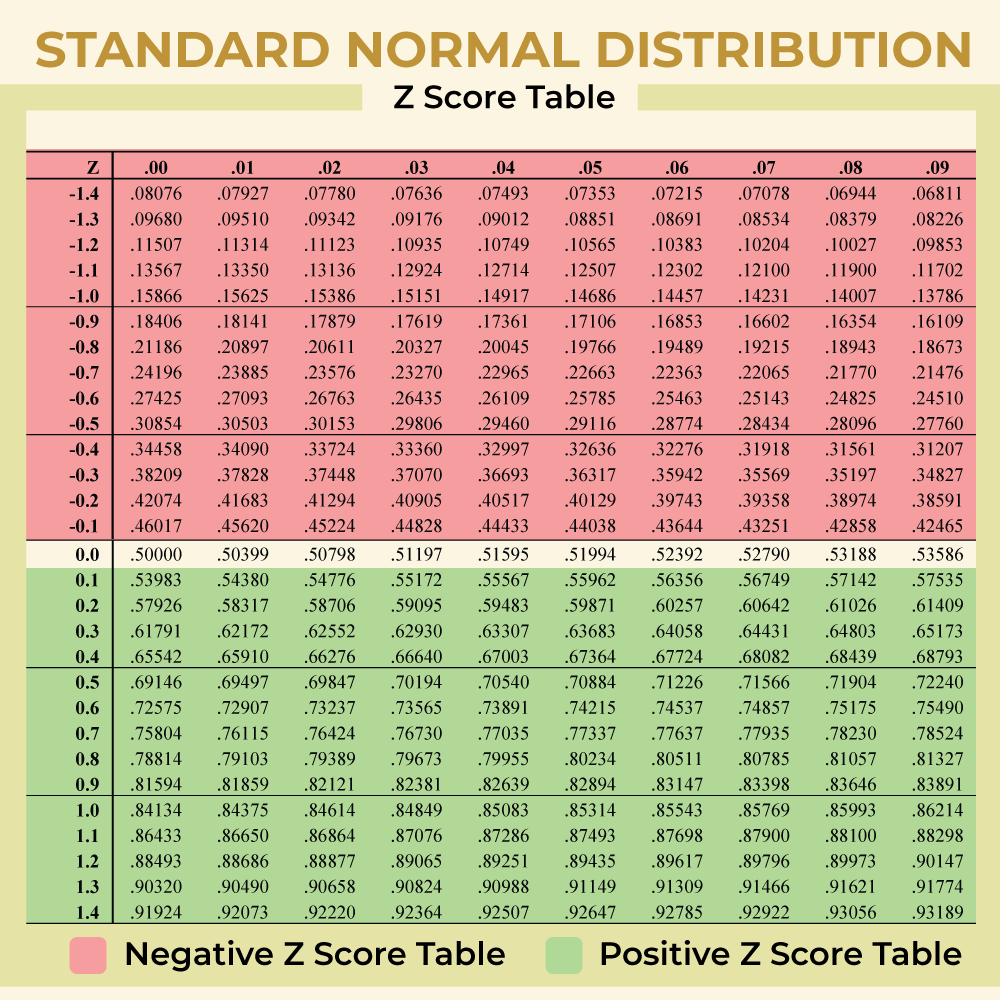
\includegraphics[width=0.70\textwidth]{Images/z-score.png}
\end{center}

Let \( X \) be the random variable representing the exam scores, where \( X \sim \mathcal{N}(72, 12^2) \).

\vspace{2mm}

\textbf{a).} To find the probability that a randomly selected student scores between 65 and 85, we need to calculate \( P(65 < X < 85) \).
We first convert the scores to z-scores:
\[ z_1 = \frac{65 - 72}{12} = -\frac{7}{12} \approx -0.5833 \]
\[ z_2 = \frac{85 - 72}{12} = \frac{13}{12} \approx 1.0833 \]
Using the z-table, we find the probabilities corresponding to these z-scores:
\[ P(Z < -0.58) \approx 0.2810 \]
\[ P(Z < 1.08) \approx 0.8599 \]
Thus, the probability that a student scores between 65 and 85 is:
\[ P(65 < X < 85) = P(Z < 1.08) - P(Z < -0.58) \approx 0.8599 - 0.2810 = 0.5789 \]
So, \( P(65 < X < 85) \approx \boxed{0.5789} \; \textbf{a).} \)

\vspace{2mm}

\textbf{b).} For a continuous random variable, the probability of scoring exactly any specific value is 0.
Thus, \( P(X = 80.00) = \boxed{0} \;\textbf{b).} \)
\end{tosubmit}
% ================================================================================ %


% ================================================================================ %
%                                    Problem 12                                    %
% ================================================================================ %
\begin{problem}
For the exam scores in Problem 11, the professor wants to give an `A' grade to the top 10\% of students.
What is the minimum score a student must get to receive an `A'?
\end{problem}

\begin{solution}
From Problem 11, we know that the exam scores follow a normal distribution: \[ X \sim \mathcal{N}(72, 12^2) \]

To find the minimum score a student must get to receive an `A',
we need to find the score corresponding to the 90th percentile of the distribution.
We first find the z-score that corresponds to the 90th percentile using the z-table: \[ z \approx 1.28 \]

We then convert this z-score back to the original score using the formula:
\[ X = \mu + z \cdot \sigma = 72 + 1.28 \cdot 12 \approx 72 + 15.36 = 87.36 \]

Thus, the minimum score a student must get to receive an `A' is approximately \( \boxed{87.36} \).
\end{solution}
% ================================================================================ %


% ================================================================================ %
%                                    Problem 13                                    %
% ================================================================================ %
\begin{problem}
Given \( Z \) is a standard normal random variable, use a Z-table to find:
\begin{subproblems}
    \item \( P(Z < -1.4) \)
    \item \( P(-0.5 < Z < 1.9) \)
\end{subproblems}
\end{problem}

\begin{solution}
\textbf{a).} From the z-table, we find:
\[ P(Z < -1.4) \approx \boxed{0.0808} \]

\textbf{b).} To find \( P(-0.5 < Z < 1.9) \), we can use the z-table to find the probabilities:
\[ P(Z < -0.5) \approx 0.3085 \text{ and } P(Z < 1.9) \approx 0.9713 \]
Thus, the probability is:
\[ P(-0.5 < Z < 1.9) = P(Z < 1.9) - P(Z < -0.5) \approx 0.9713 - 0.3085 = \boxed{0.6628} \]
\end{solution}
% ================================================================================ %


% ================================================================================ %
%                                    Problem 14                                    %
% ================================================================================ %
\begin{problem}
Find the value of \( c \) for a standard normal variable \( Z \) such that:
\begin{subproblems}
    \item \( P(Z < c) = 0.99 \)
    \item \( P(Z > c) = 0.75 \)
\end{subproblems}
\end{problem}

\begin{solution}
\textbf{a).} From the z-table, we find:
\[ P(Z < c) = 0.99 \Rightarrow c \approx \boxed{2.3} \]

\textbf{b).} To find \( P(Z > c) = 0.75 \), we can use the z-table to find the corresponding z-score:
\[ P(Z < c) = 1 - P(Z > c) = 1 - 0.75 = 0.25 \Rightarrow c \approx \boxed{-0.7} \]
\end{solution}
% ================================================================================ %

\newpage

% ================================================================================ %
%                                    Problem 15                                    %
% ================================================================================ %
\begin{problem}
The weight of coffee in a ``large'' cup from a machine is \( X \sim \mathcal{N}(400, 100) \) (in ml).
The weight of milk added is \( Y \sim \mathcal{N}(50, 25) \). Assume \( X \) and \( Y \) are independent.
\begin{subproblems}
    \item Let \( T = X + Y \) be the total volume. What are \( \text{E}[T] \) and \( \text{Var}(T) \)?
    \item  What is the probability the total volume exceeds 460 ml?
\end{subproblems}
\end{problem}

\begin{solution}
\textbf{a).} For independent random variables \( X \) and \( Y \):
\[ \text{E}[T] = \text{E}[X] + \text{E}[Y] = 400 + 50 = \boxed{450 \text{ ml}} \]
\[ \text{Var}(T) = \text{Var}(X) + \text{Var}(Y) = 100 + 25 = \boxed{125 \text{ ml}^2} \]

\textbf{b).} To find the probability that the total volume exceeds 460 ml, we first find the distribution of \( T \):
\[ T \sim \mathcal{N}(450, 125) \]
We need to calculate \( P(T > 460) \). We first convert this to a z-score:
\[ z = \frac{460 - 450}{\sqrt{125}} = \frac{10}{\sqrt{125}} \approx 0.9 \]
Using the z-table, we find:
\[ P(Z < 0.9) \approx 0.8159 \]
Thus, the probability that the total volume exceeds 460 ml is:
\[ P(T > 460) = 1 - P(Z < 0.9) \approx 1 - 0.8159 = \boxed{0.1841} \]
\end{solution}
% ================================================================================ %


% ================================================================================ %
%                                    Problem 16                                    %
% ================================================================================ %
\begin{problem}
\end{problem}

\begin{solution}
Let \( D = B - C \). Since \( B \) and \( C \) are independent normal random variables, \( D \) is also normally distributed:
\[ D \sim \mathcal{N}(\text{E}[B] - \text{E}[C], \text{Var}(B) + \text{Var}(C)) \]
Calculating the mean and variance of \( D \):
\[ \text{E}[D] = 120 - 125 = -5 \]
\[ \text{Var}(D) = 16 + 9 = 25 \]
Thus, \( D \sim \mathcal{N}(-5, 25) \).

We need to find \( P(D > 0) \), which is equivalent to finding \( P(B > C) \).
We first convert this to a z-score:
\[ z = \frac{0 - (-5)}{\sqrt{25}} = \frac{5}{5} = 1 \]
Using the z-table, we find:
\[ P(Z < 1) \approx 0.8413 \]
Thus, the probability that the blueberry muffin is heavier than the chocolate chip muffin is:
\[ P(D > 0) = 1 - P(Z < 1) \approx 1 - 0.8413 = \boxed{0.1587} \]
\end{solution}
% ================================================================================ %

\newpage

% ================================================================================ %
%                                    Problem 16                                    %
% ================================================================================ %
\begin{problem}
Let \( X \) be a random variable representing the outcome of a fair six-sided die roll.
Let \( Y \) be a continuous random variable from a \( U(1, 6) \) distribution.
\begin{subproblems}
    \item Explain the fundamental difference between \( P(X = 4) \) and \( P(Y = 4) \).
    \item Calculate \( P(X > 4) \) and \( P(Y > 4) \).
\end{subproblems}
\end{problem}

\begin{solution}
\textbf{a).} The fundamental difference between \( P(X = 4) \) and \( P(Y = 4) \) lies in the nature of the random variables.

\vspace{2mm}

\( X \) is a discrete random variable, meaning it can take on specific, countable values (in this case, the integers 1 through 6).
Therefore, \( P(X = 4) \) represents the probability of rolling a 4 on a fair six-sided die, which is a non-zero value:
\[ P(X = 4) = \frac{1}{6} \]

\vspace{2mm}

On the other hand, \( Y \) is a continuous random variable, meaning it can take on any value within a given range (in this case, between 1 and 6).
For continuous random variables, the probability of taking on any specific value is zero. Therefore,
\[ P(Y = 4) = 0 \]

\textbf{b).} To calculate \( P(X > 4) \) for the discrete random variable \( X \):
\[ P(X > 4) = P(X = 5) + P(X = 6) = \frac{1}{6} + \frac{1}{6} = \frac{2}{6} = \frac{1}{3} \]
To calculate \( P(Y > 4) \) for the continuous random variable \( Y \):
The PDF of a uniform distribution \( U(a, b) \) is given by:
\[ f_Y(y) = \begin{cases}
    \frac{1}{b-a} & a \leq y \leq b \\
    0 & \text{otherwise}
\end{cases} \]
For our case, \( a = 1 \) and \( b = 6 \), so the PDF is:
\[ f_Y(y) = \begin{cases}
    \frac{1}{5} & 1 \leq y \leq 6 \\
    0 & \text{otherwise}
\end{cases} \]
To find \( P(Y > 4) \), we can integrate the PDF from 4 to 6:
\[ P(Y > 4) = \int_{4}^{6} f_Y(y) \, dy = \int_{4}^{6} \frac{1}{5} \, dy = \frac{1}{5} \cdot (6 - 4) = \frac{2}{5} \]
Thus, \( P(X > 4) = \frac{1}{3} \) and \( P(Y > 4) = \frac{2}{5} \).
\[\boxed{P(X > 4) = \frac{1}{3}, \; P(Y > 4) = \frac{2}{5}}\]
\end{solution}
% ================================================================================ %

\newpage

% ================================================================================ %
%                                    Problem 18                                    %
% ================================================================================ %
\begin{problem}
Suppose \( X \sim U(0, 1) \). Let a new random variable be defined as \( Y = -\ln(X) \).
Find the PDF of \( Y \), \( f_Y(y) \). What famous distribution is this?
\end{problem}

\begin{solution}
To find the PDF of \( Y \), we can use the method of transformation. The CDF of \( Y \) is given by:
\[
F_Y(y) = P(Y \leq y) = P(-\ln(X) \leq y) = P(X \geq e^{-y}) = 1 - P(X < e^{-y}) = 1 - e^{-y}
\]
for \( y \geq 0 \).

Differentiating the CDF gives us the PDF:
\[
\boxed{f_Y(y) = \frac{d}{dy} F_Y(y) = e^{-y}} \; \text{for } y \geq 0
\]

This is the PDF of the exponential distribution with parameter \( \lambda = 1 \). Thus, \( Y \) follows an exponential distribution:
\[
\boxed{Y \sim \text{Exponential}(1)}
\]
\end{solution}
% ================================================================================ %


% ================================================================================ %
%                                    Problem 19                                    %
% ================================================================================ %
\begin{problem}
A factory produces widgets, and 5\% are defective. You take a random sample of 500 widgets.
Use the normal approximation to the binomial distribution to estimate the probability that you will find 30 or more defective widgets in your sample.
(Remember to use the continuity correction).
\end{problem}

\begin{solution}
Let \( X \) be the number of defective widgets in the sample. Then \( X \sim \text{Binomial}(n=500, p=0.05) \).
The mean and variance of \( X \) are:
\[ \text{E}[X] = np = 500 \times 0.05 = 25 \]
\[ \text{Var}(X) = np(1-p) = 500 \times 0.05 \times 0.95 = 23.75 \]

Using the normal approximation, we can approximate \( X \) with a normal distribution:
\[ X \sim \mathcal{N}(25, 23.75) \]
To find the probability of finding \underline{30 or more} defective widgets, we use the continuity correction:
\[ P(X \geq 30) \approx P(X > 29.5) \]
We convert this to a z-score:
\[ z = \frac{29.5 - 25}{\sqrt{23.75}} \approx \frac{4.5}{4.873} \approx 0.92 \]
Using the z-table, we find:
\[ P(Z < 0.92) \approx 0.81859 \]
Thus, the probability of finding 30 or more defective widgets is:
\[ P(X \geq 30) = 1 - P(Z < 0.92) \approx 1 - 0.81859 = \boxed{0.18141} \]
\end{solution}
% ================================================================================ %

\newpage

% ================================================================================ %
%                                    Problem 20                                    %
% ================================================================================ %
\begin{problem}
The time \( T \) (in minutes) to solve a complex puzzle follows an exponential distribution with a parameter \( \lambda = 1/15 \).
If a player is paid based on their time according to the function \( P(T) = 100 - 2T \) dollars, what is the expected payout?
\end{problem}

\begin{solution}
The expected payout can be calculated using the formula:
\[ \text{E}[P(T)] = \int_{0}^{\infty} P(t) f_T(t) \, dt \]
where \( f_T(t) = \lambda e^{-\lambda t} \) is the PDF of the exponential distribution.

Given \( \lambda = \frac{1}{15} \), the PDF is:
\[ f_T(t) = \frac{1}{15} e^{-\frac{t}{15}} \text{ for } t \geq 0 \]

Substituting \( P(t) \) and \( f_T(t) \) into the expected payout formula:
\begin{align*}
    \text{E}[P(T)] &= \int_{0}^{\infty} (100 - 2t) \cdot \frac{1}{15} e^{-\frac{t}{15}} \, dt \\
    &= \frac{1}{15} \int_{0}^{\infty} (100 - 2t) e^{-\frac{t}{15}} \, dt \\
    &= \frac{1}{15} \paren{100 \int_{0}^{\infty} e^{-\frac{t}{15}} \, dt - 2 \int_{0}^{\infty} t e^{-\frac{t}{15}} \, dt} \\
    &= \frac{1}{15} \paren{100 \sqbracket{-15e^{-\frac{t}{15}}}_{0}^{\infty} - 2 \sqbracket{-15te^{-\frac{t}{15}} - 225e^{-\frac{t}{15}}}_{0}^{\infty}} \\
    &= \frac{1}{15} \paren{100 \sqbracket{0 - (-15)} - 2 \sqbracket{(0 - 0) - (0 - 225)}} \\
    &= \frac{1}{15} \paren{100 \cdot 15 - 2 \cdot 225} \\
    &= \frac{1}{15} \paren{1500 - 450} \\
    &= \frac{1050}{15} \\
    \text{E}[P(T)] &= 70
\end{align*}

Thus, the expected payout is \( \boxed{70 \text{ dollars}} \).
\end{solution}
% ================================================================================ %

\vspace{1.5cm}

\zScoreTable{1.2}

\end{document}